\documentclass{article}

% if you need to pass options to natbib, use, e.g.:
% \PassOptionsToPackage{numbers, compress}{natbib}
% before loading nips_2018

% ready for submission
\usepackage{nips_2018}
\usepackage{graphicx}
\usepackage{caption}
\usepackage{subcaption}

% to compile a preprint version, e.g., for submission to arXiv, add
% add the [preprint] option:
% \usepackage[preprint]{nips_2018}

% to compile a camera-ready version, add the [final] option, e.g.:
% \usepackage[final]{nips_2018}

% to avoid loading the natbib package, add option nonatbib:
% \usepackage[nonatbib]{nips_2018}

\usepackage[utf8]{inputenc} % allow utf-8 input
\usepackage[T1]{fontenc}    % use 8-bit T1 fonts
\usepackage{hyperref}       % hyperlinks
\usepackage{url}            % simple URL typesetting
\usepackage{booktabs}       % professional-quality tables
\usepackage{amsfonts}       % blackboard math symbols
\usepackage{nicefrac}       % compact symbols for 1/2, etc.
\usepackage{microtype}      % microtypography

\title{Yelp Dataset Review Rating Prediction Analysis}

% The \author macro works with any number of authors. There are two
% commands used to separate the names and addresses of multiple
% authors: \And and \AND.
%
% Using \And between authors leaves it to LaTeX to determine where to
% break the lines. Using \AND forces a line break at that point. So,
% if LaTeX puts 3 of 4 authors names on the first line, and the last
% on the second line, try using \AND instead of \And before the third
% author name.

\author{
  Shihao Lin \\
  Pitzer College\\
  1050 N. Mills. Ave, CA 91711 \\
  \texttt{shilin@pitzer.students.edu} \\
  \\
   \textbf{Ziyuan Shang} \\
   Scripps College\\
   Claremont,CA,91711 \\
   \texttt{zshang9431@scrippscollege.edu} \\
 }


\begin{document}
% \nipsfinalcopy is no longer used

\maketitle
\begin{abstract}
  Rating prediction is one of the most important
application of machine learning. In this project, 
we explore the Yelp dataset and are looking for appropriate machine learning algorithms to predict the star users will assign to a business through the content of review they wrote. We use the basic topic modeling processed the data and use classification algorithms like Naive Bayes(NB) algorithm, MultinomialNB, BernoulliNB, Logistic Regression and Linear Support Vector Machine to do binary classification (positive and negative) on the dataset. Using Tf-idf vectorizer and bigram model, our highest accuracy reached 98.16\%. 
\end{abstract}

\section{Introduction}
Yelp is an American multinational corporation headquartered in San Francisco, California. It was founded in 2004, and dedicated to helping people find a great local business like restaurants and hair salons. The company allows users to give star ratings and write reviews for the business. More than 155 millions of reviews have been written by Yelp users by the end of Q1 2018. Among these reviews, myriads of hidden information can be extracted, and this information can be beneficial to business owners as well as customers. By studying these reviews, owners can be more aware of things that they need to improve, and customers will be able to find better matches for their own tastes. However, how to extract the most important information has remained a big challenge for a long time. The project specifically focuses on building a model that can extract useful features from millions of reviews. Processing these reviews using sentiment analysis, finding the most featured words and predicting the proper ratings solely based on review text.

\section{Data description}

Yelp's datasets include six files, which are business.json, review.json, user.json, checkin.json, tip.json, and photos. In our midterm modeling, we used the business.json and review. json. Later, we will further explore the review.json for our final modeling. In the following subsections, we are going to illustrate the datasets and its format.

In this dataset, the total organizations are 146702, the total users are 1326101, the total reviews are 1493480, the total negative reviews (from rating scale 0 to 4) are 504771, and total positive reviews (from rating scale 4 to 5) are 988709. 

\begin{figure}[!ht]
\centering
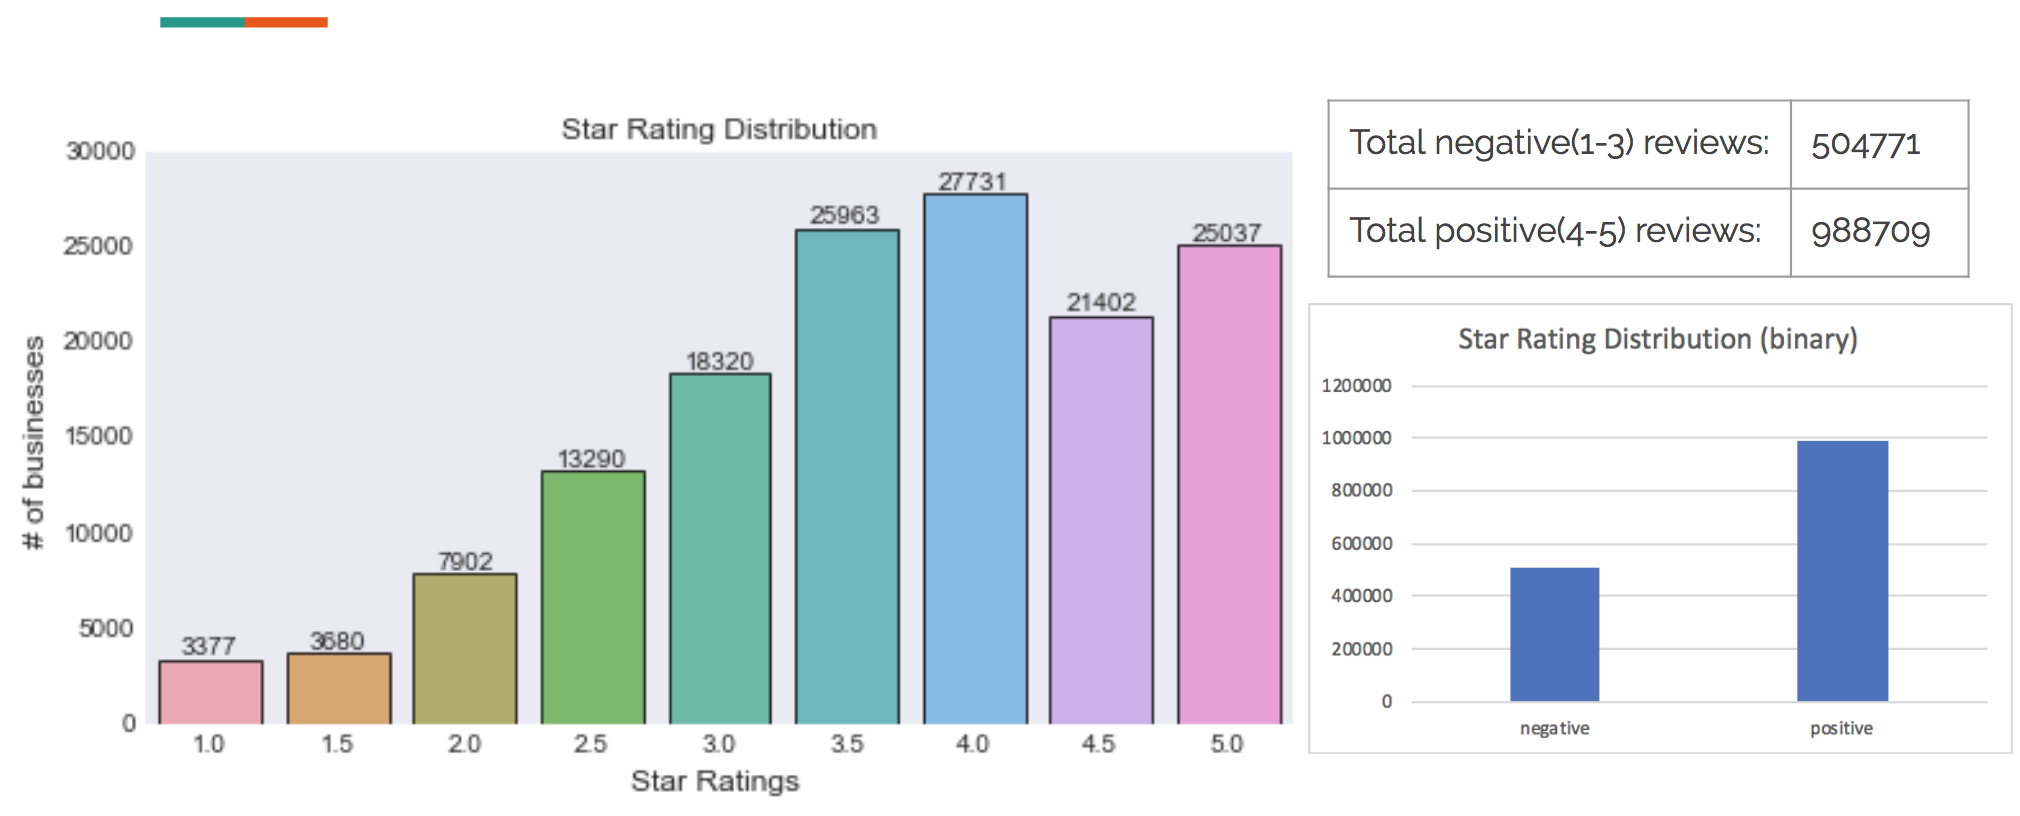
\includegraphics[width=\textwidth]{ReviewDistribution.png}
\caption{Star Rating Distribution}
\end{figure}

The above figure 1 illustrates the review star distribution. Based on figure 1, we can notice that the total start reviews are mostly made up by positive reviews.

\subsection{Files Description}

The file Business.json contains business data including location data, attributes, and categories. More specific, this file includes information of city, state, latitude, and longitude of the store, stars, review counts, business parking, ambience, price level, Good for meal and etc. In the later section, we would set up the model to illustrate the correlations between all of those attributes and business rating. In other words, we are going to build up a model to predict the business rating applying some of the features to different types of existing algorithms to train the computer.

The file Review.json contains full review text data including the user\_id that wrote the review and the business\_id the review is written for. We will not use this for the midterm report. But we will use this file for the final modeling to predict a solo review star, which is based on its review text.

\section{Data Analysis}
Before we actually start analyzing the data, we transform the format from json to csv, which is convenient for us to analyze the data. In the following subsections, we generate various graphs to help visualize the relationship between different feature.

\subsection{Location v.s Review counts}
In the first part, we link the review counts to states. We find out that Arizona has the most reviews, which is a bit surprising. The topmost reviews states are Arizona, Nevada, Oregon, North Carolina, and Ohio. Surprisingly, we find that California is not on this list. 
\begin{figure}[!ht]
\centering
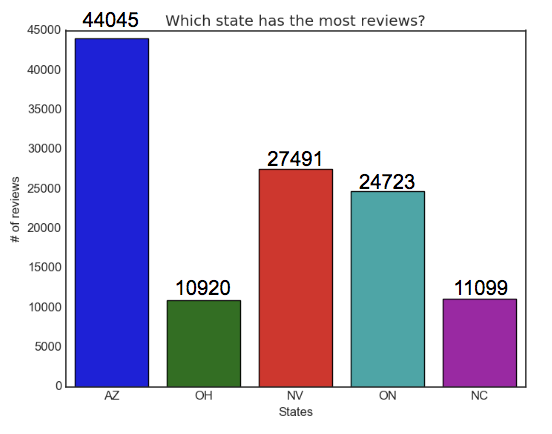
\includegraphics[width=10cm]{state.png}
\caption{What state has the most reviews?}
\end{figure}
We also link the review counts to the city. We find that Las Vegas has the most reviews, which is 22113 and is also the main component of the total reviews of Nevada. The following figure 2 illustrates the topmost reviews city in the U.S.
\begin{figure}[!ht]
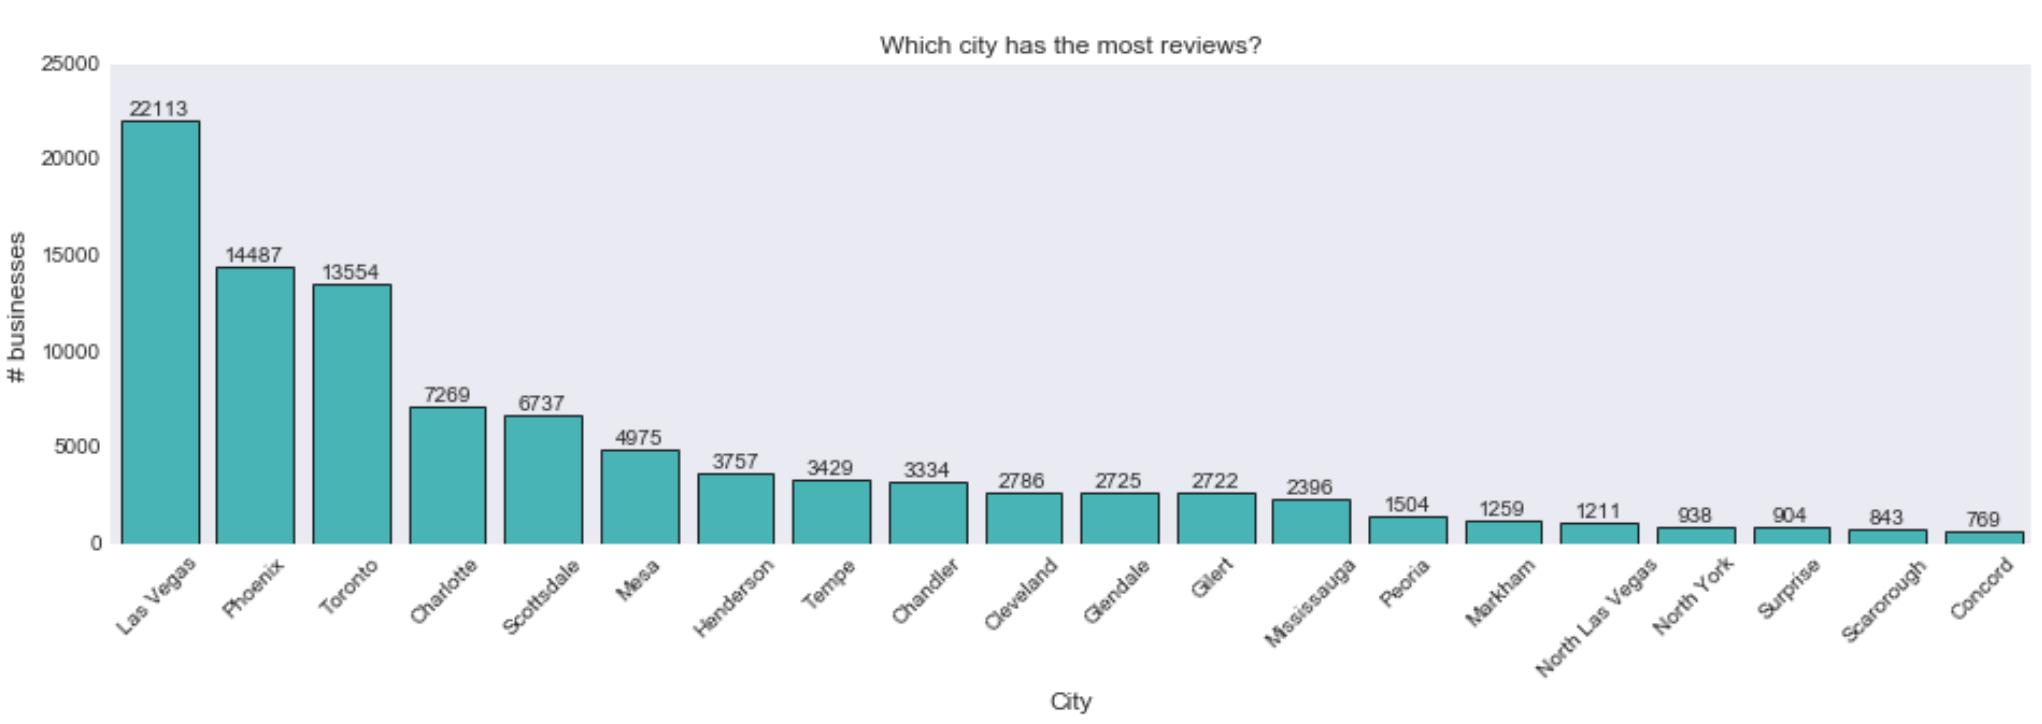
\includegraphics[width=\textwidth]{City.png}
\caption{Which city has the most reviews}
\end{figure}
By using the latitudes and longitudes of business organizations and its review counts, we can plot out a graph about that information, just like the following figure 3 about Las Vegas and Phoenix. Each review will represent a small black dot. The more reviews in the same location, the dot will be darker. Therefore, we can use this graph to predict where is the most popular place in a city.
\begin{figure}[!ht]
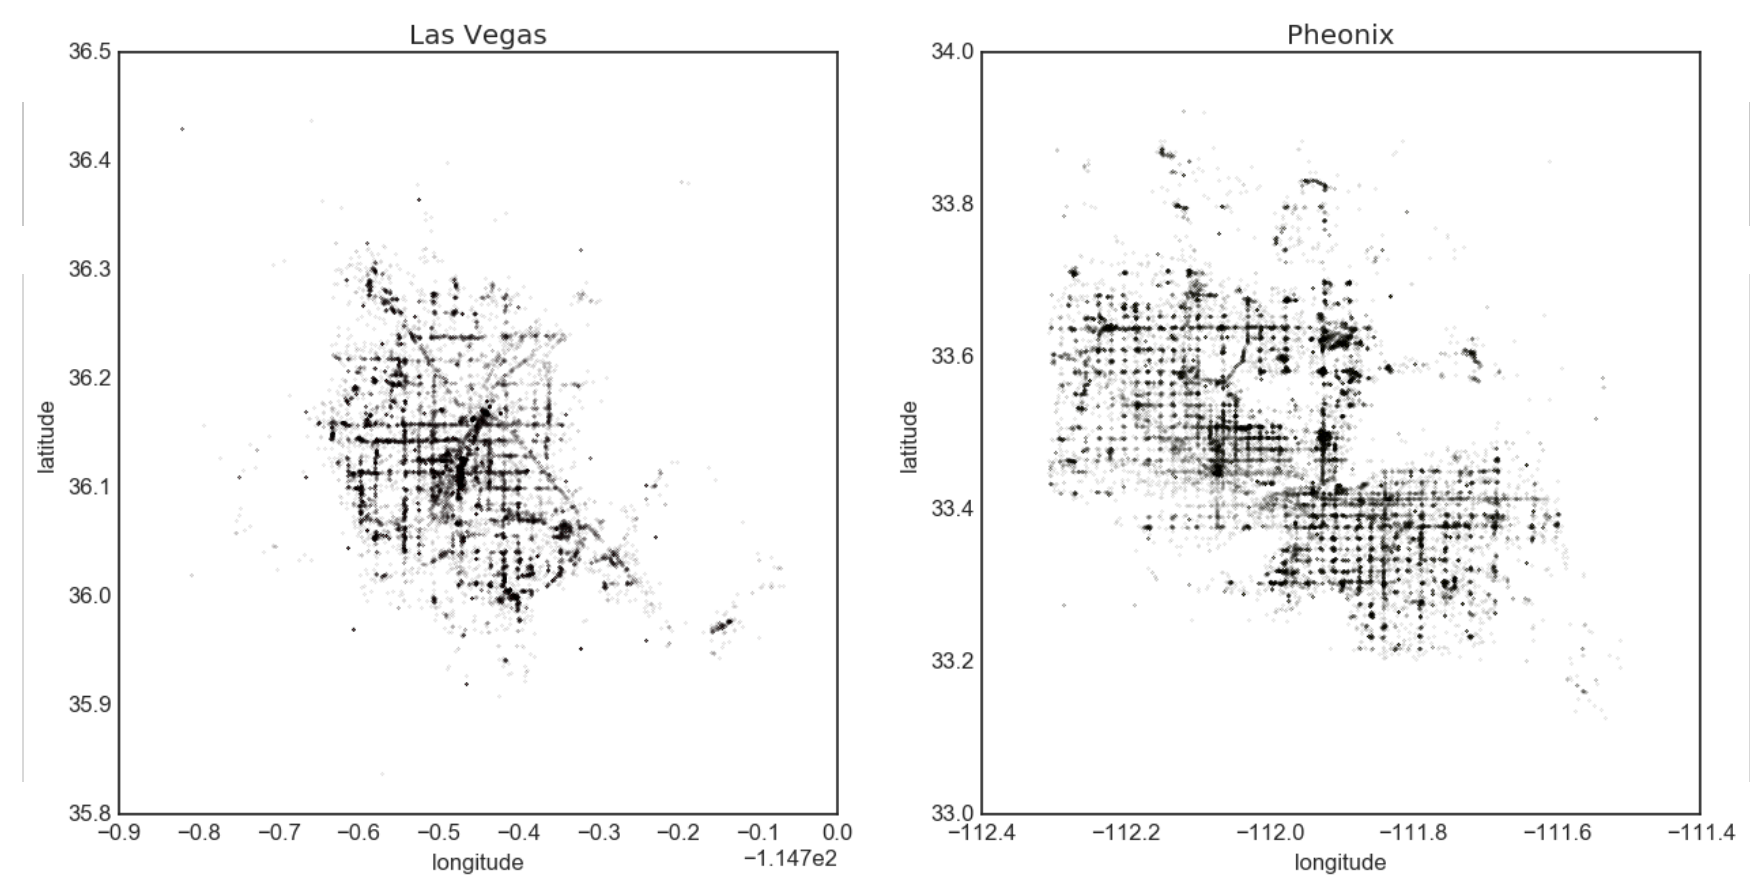
\includegraphics[width=\textwidth]{Graph.png}
\caption{Business popularity on city map}
\end{figure}

\subsection{Review Count v.s. rating}

\begin{figure}[t]
\centering
\begin{minipage}{.5\textwidth}
  \centering
  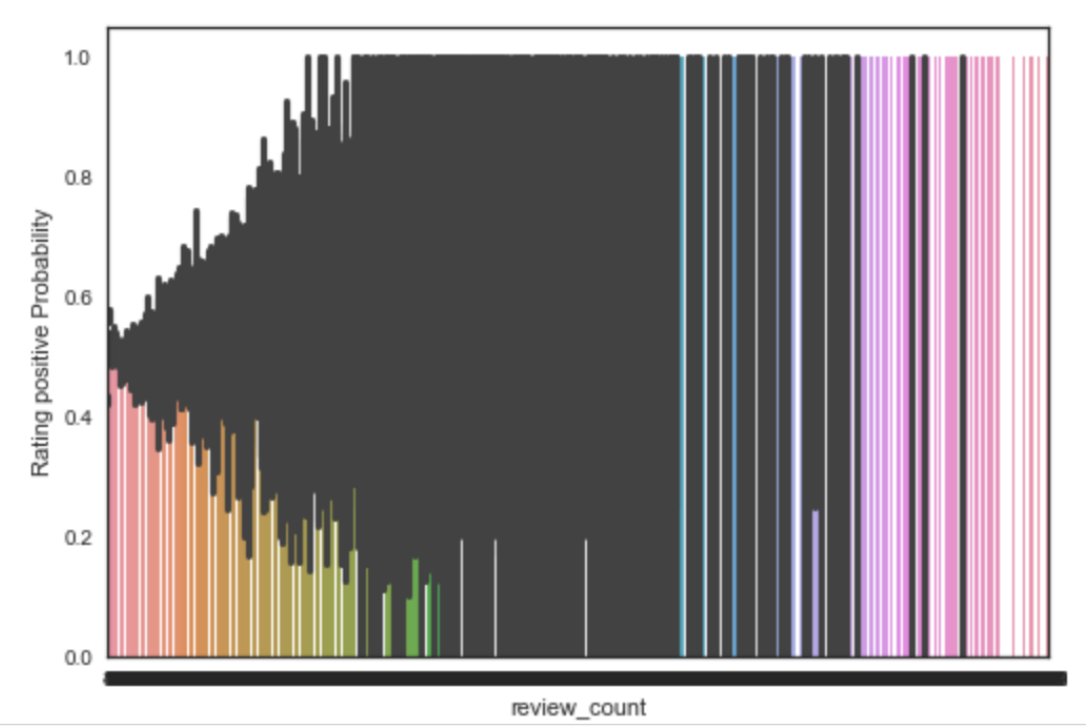
\includegraphics[width=\linewidth]{ReviewvR.png}
  \captionof{figure}{Review Count v.s. Rating}
  \label{fig:test1}
\end{minipage}%
\begin{minipage}{.5\textwidth}
  \centering
  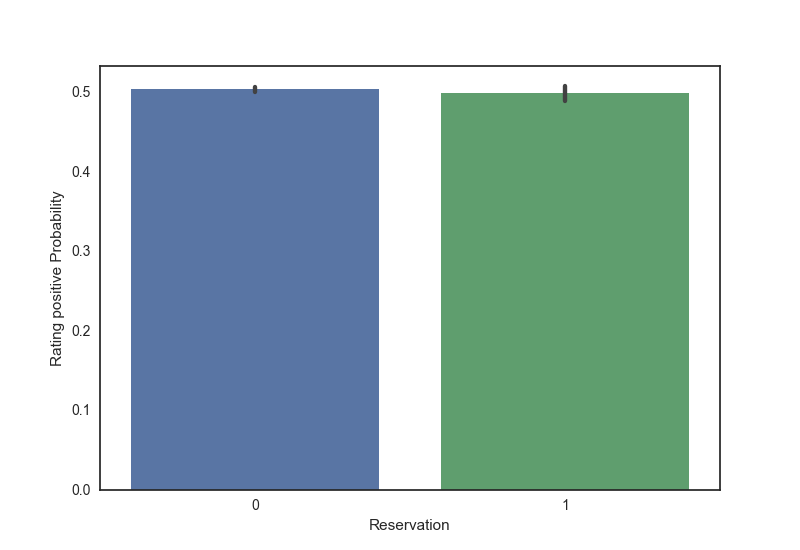
\includegraphics[width=\linewidth]{Reservation}
  \captionof{figure}{Reservation v.s Rating}
  \label{fig:test2}
\end{minipage}
\end{figure}

In figure 4 "Review count v.s. Rating", we label the number of review in one single business organization into horizontal axis, and the probability to get a positive review into vertical axis. We found that if a business has fewer reviews, the probability of it to be rated as positive is around 50\%. The business organization with a medium amount of review tends to have high variance on its probability to be rated as positive. The organization with large reviews often tend to have the probability to be rated as positive.

\subsection{Reservation v.s. Rating}
We want to discover the relationship between whether an organization accepts reservation would influence it to be rated as positive. Therefore, we analyzed the data and put it into a histogram as presented in figure 5. On the horizontal axis, 0 represents that reservation service is unavailable, and 1 represents that reservation service is available. The vertical axis shows the probability for each type of organization to be rated as positive. As a result, we found the probability of being rate as positive for both types are very similar and centering around 50 percentage. Thus, we conclude that there is no such correlation between the service of reservation and business rating. 

\subsection{Price v.s. Rating}

\begin{figure}[t]
\centering
\begin{minipage}{.5\textwidth}
  \centering
  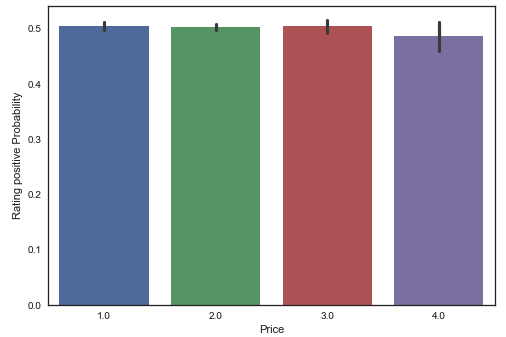
\includegraphics[width=\linewidth]{Price.png}
  \captionof{figure}{Price v.s. Rating}
  \label{fig:test1}
\end{minipage}%
\begin{minipage}{.5\textwidth}
  \centering
  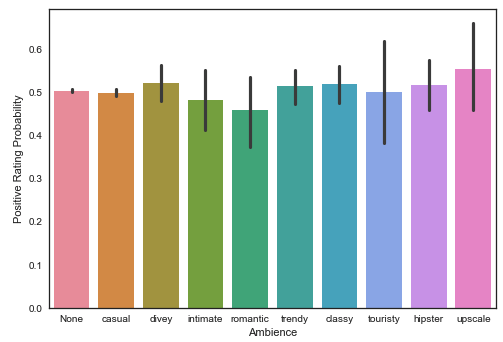
\includegraphics[width=\linewidth]{Ambience.png}
  \captionof{figure}{Ambience v.s Rating}
  \label{fig:test2}
\end{minipage}
\end{figure}

The price level of a restaurant is always a big factor to influence people's decision of selecting a restaurant. Sometime, people would think an expensive restaurant tend to taste better than a cheap restaurant. In this paper, we are going to present our finding of the correlation between price level and business rating. By plugging the price level data and business rating data into "Seaborn" analyzer, we get a histogram in figure 6. Each number on the horizontal axis represents different price levels. "1.0" means very cheap, and "4.0" means very expensive. The vertical axis shows the probability for different price levels of an organization to be rated as positive. As a result, we found the probability of all four different price level are very similar and close to 50 percentage, and the probability of price level 4 is slightly lower than the price level. Thus, the result indicates the price level may not have much influence on Business Rating. A very expensive restaurant may not always taste very good.

\subsection{Ambience v.s. Rating}

Different type ambience of a restaurant tends to have different chance to be rated as a positive good restaurant. We want to discover the correlation between ambience and rating. In the yelp dataset, it provides 10 categories for ambience, "None", "casual", "divey","intimate","romantic", "trendy","classy",'touristy", "hipster", and "upscale". Then we plugged all of those data with its business rating into "Seaborn" analyzer. We get a bar diagram in figure 7. Different categories are labeled in the horizontal axis. The vertical axis shows the probability for different categories of an organization to be rated as positive. As we observed, "upscale" ambience restaurant tend to have higher chance to be rated as positive. However, in general, since the positive rating probability for all categories is all laid between 40 percentage and 60 percentage, the ambience does not seem to have much correlation with the business rating.

\subsection{City v.s. Rating}
\begin{figure}[t]
\centering
\begin{minipage}{.5\textwidth}
  \centering
  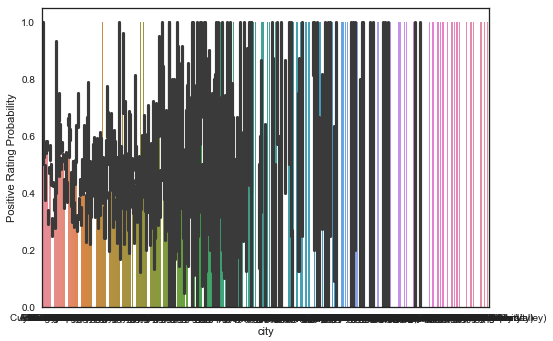
\includegraphics[width=\linewidth]{CityR.png}
  \captionof{figure}{City v.s. Rating}
  \label{fig:test1}
\end{minipage}%
\begin{minipage}{.5\textwidth}
  \centering
  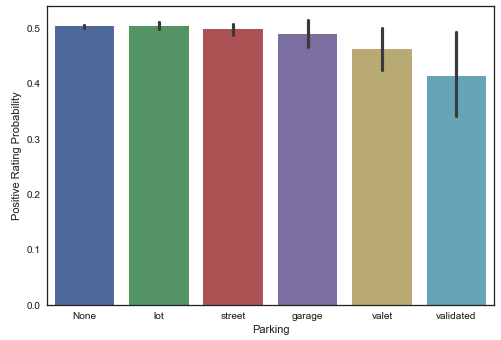
\includegraphics[width=\linewidth]{Parking.png}
  \captionof{figure}{Parking v.s Rating}
  \label{fig:test2}
\end{minipage}
\end{figure}
We are curious about whether the overall quality of food in some city is higher than other cities. Therefore, we input all organizations' city location and corresponding business rating into "Seaborn" analyzer and get a histogram as shown in figure 8. The cities' names are labeled in a horizontal axis, and the corresponding positive rating probability is presented by a vertical axis. The different color bar represents the different city, and the black bar is the variance of the probability. By observation, we found some city definitely have higher overall quality restaurant than others.

\subsection{Parking v.s. Rating}

The transportation in most of the place in the U.S. is driving. In average, every household has around 2 cars in the U.S. Thus, we think whether a restaurant would provide parking service is essential to its rating. Then we plug the data about its restaurant parking situation and corresponding business rating into "Seaborn" analyzer and get a histogram. As in figure 9, we observe that the positive rating probability for all categories is under 50 percent. Thus, the service of parking does not seem to have much influence on the business rating. 

\subsection{Good For Meal v.s. Rating}
\begin{figure}[t]
\begin{minipage}{.5\textwidth}
  \centering
  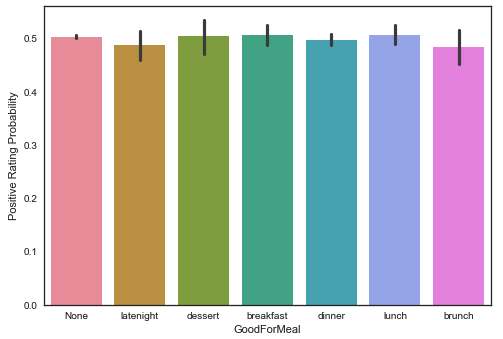
\includegraphics[width=\linewidth]{GFN.png}
	\caption{Good For Meal v.s Rating}
    \end{minipage}
\begin{minipage}{.5\textwidth}
	\centering
    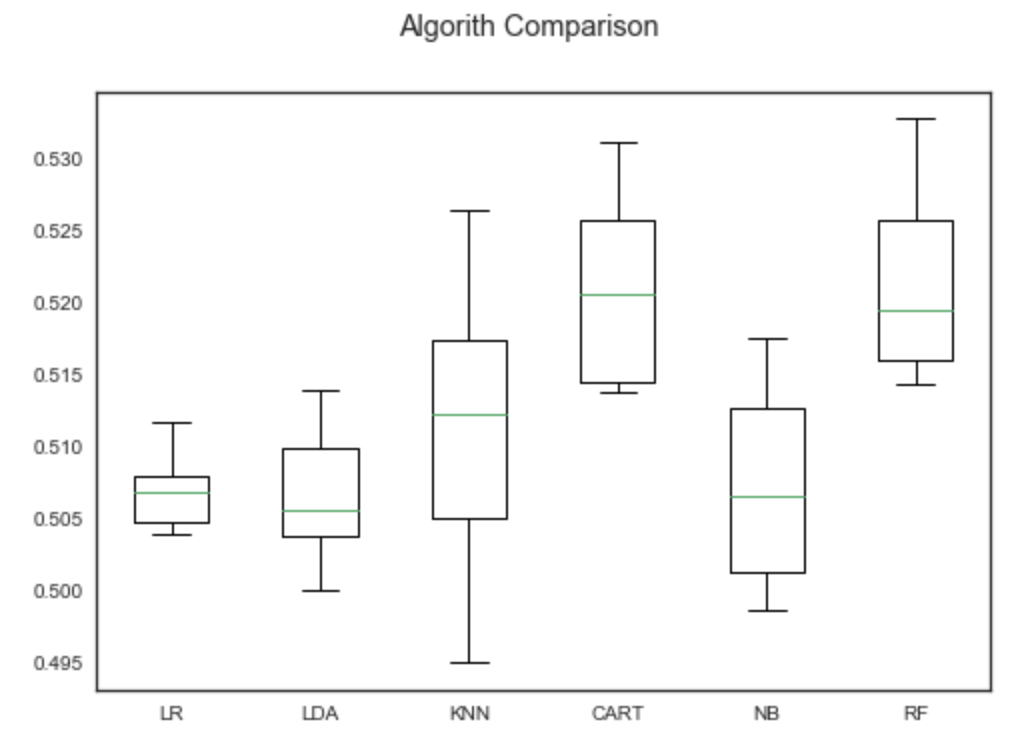
\includegraphics[width=\linewidth]{Algorithm.png}
    \caption{Algorithm.png}
\end{minipage}
\end{figure}
At first, we consider that different meal type may have an influence on the business rating. For example, restaurant, which focuses on making breakfast, in general, may have higher business rating than those focuses on making brunch. In yelp data, it provides 7 categories for "Good For Meal", which are "None", "late night", "dessert", "breakfast", "dinner", "lunch", and "brunch". While we plugged all of those data and corresponding business rating, we get a bar diagram, as shown in figure 10. The meal categories are labeled in a horizontal axis, and the corresponding positive rating probability is presented by a vertical axis. By observation, we found that the positive rating probability for all categories are very similar and around 50 percentage. Thus, distinguishing meal specialty of a restaurant may not help to distinguish its business rating.

\section{Business Analysis}

Before actually applying the data into the algorithm, we decide to filter out some features of the dataset. In the end, we remain the three features, review\_count  Reservation, and Parking, to predict the business rating. We set 75 percentage dataset as the training dataset, and remain 25 percentage dataset as the testing dataset. Then we purposely select six different methods to predict the outcome, which is "Logistic Regression", "Linear Discriminant Analysis", "K-Neighbors Classifier", "Decision Tree Classifier", "Gaussian Naive Bayes", and "Random Forest Classifier" from $sklearn$ package. All of six methods could be used to analyze a binary outcome.

In the previous section, although the features in the dataset are independence to each other, we notice that most of the features in this dataset do not have much correlation with the business rating. Therefore, we assume that the accuracy for those algorithms to have a right prediction is low. The overall result is present in the following table, and the visualized version is in figure 12.

By observation, the overall accuracy is very low and around 50 percentage. We observed that " Logistic regression" method has the lowest variance, "K-nearest Neighbors classifier" has the highest variance, and "Random Forest classifier" brings up the highest accuracy, which is yielding roughly 52.11\%. Although "Decision tree classifier" is the underlying concept for "Random Forest classifier", the accuracy performance does not have much different.   In conclusion, the correlation between the feature and its outcome is essential for generating a high accuracy prediction.

\begin{table}[!ht]
\begin{center}
\begin{tabular}{ |c|c| } 
 \hline
Algorithm & Accuracy Percentage \\ 
  \hline
Logistic\_Regression\_classifier & 0.506369 (0.003203) \\ 
  \hline
Linear\_Discriminant\_Analysis & 0.506685 (0.004129) \\
  \hline
K-Neighbors\_classifier & 0.511014 (0.009426) \\
  \hline
Decision\_Tree\_classifier & 0.520832 (0.006517) \\
  \hline
Gaussian\_Naive\_Bayes & 0.506978 (0.006656) \\
  \hline
Random\_Forest\_classifier & 0.521114 (0.006188) \\
\hline
\end{tabular}
\end{center}
\end{table}

\section{Review Analysis}
In our review analysis, we mainly explored the relationship between review content (what words does user use) and rating of the corresponding business. We first attempted our reviews analysis on a smaller sample. Form our reviews dataset, we generated a random sample of 3000 reviews. We will scale the code to perform analysis for the entire dataset in the future. 

\subsection{Data preparation}
The data used in this analysis comes from the preprocessed review.csv mentioned in Section 3. The only useful columns are \textit{text} - the actual review content given by the user in a string format, and  \textit{review\_stars} - the star rating associated with the review. A third column named \textit{Rating} is created based on \textit{review\_stars} - reviews with 1, 2 stars are considered negative; reviews with 4 or 5 stars are considered positive.

\subsection{Feature selection} 
Prior to fitting the model and using machine learning algorithms for training, we need to represent the text document as a feature vector. A commonly used model in Natural Language Processing is the \textit{bag of words} model. It first comes the creation of the vocabulary — the collection of all different words that occur in the training set and each word is associated with a count of how it occurs. The vocabulary can then be used to construct the d-dimensional feature vectors for the individual documents where the dimensionality is equal to the number of different words in the vocabulary. Before we do the vectorization, we need to pre-processing the code.  

\subsubsection{Text pre-processing}
First, we performed several necessary pre-processing on review test, including tokenizing, removing stop words and stemming.

Tokenizing refers to the act of separating a sentence into individual word tokens. In our analysis, we used the default \textit{word\_tokenizer} in the \textit{nltk} package under Python. As an example, if we pass the following sentence:"The python programmer named pythoner is pythoning a game pythonly." into the \textit{word\_tokenizer}, the returned result will be 
\['The','python','programmer', 'named', 'pythoner', 'is', 'pythoning', 'a', 'game', 'pythonly'\] 
After tokenization, we need to remove the common stop words in English. Stop words are words that appear extremely common but do not convey much meaning or sentiment of bodies of text. We used the bad of stop words gathered by the \textit{nltk} package and eliminated the words that falls into this bag from each piece of text. Using the above example, after removing the stop words, the returned result is 
\['The','python','programmer', 'named', 'pythoner', 'pythoning', 'game', 'pythonly'\] 
Observed that the words 'is' and 'a' are removed from the list, whereas the words that conveying meanings are kept. 

Then we stemmed the individual words in each piece of text using Porter Stemmer(C.J. van Rijsbergen and Porter,1980). Stemming refers to "the process of reducing inflected (or sometimes derived) words to their word stem, base or root from generally a written word form". In particular, Porter Stemmer is the de facto algorithm developed in 1980, and it was widely used to stem English words. In our analysis, we used the \textit{nltk} implementation of Porter Stemmer to bring words from text to its stem form. Here, we assumed that words with the same stem convey roughly the same meaning, and therefore are weighted equally in sentiment analysis. 

After passing the above list to a Porter Stemmer, the list returned is in the following form: 
\['the','python','programm', 'name', 'python', 'python', 'game', 'pythonli'\]
Observed that all python-related words, except 'pythonly', are being turned into its stemmed for 'python'. The single exception of the adverb might be an example of under stemming. 

\subsubsection{Spare Matrix Representation}
The final step towards model training is transforming the body of text into a spare matrix representation. We have explored two different ways: Count Vectorizer and Tf-idf Vectorizer. 

The idea behind Count Vectorizer is quite simple: we first identify all the unique words that are present in all of the review, then create a matrix whose columns are individual words and rows are individual documents. The values represent the number of times the word appeared. 
Let $D_1$ and $D_2$ be two documents in a training dataset: $D_1$:"Each state has its own laws.";
$D_2$:"Each country has its own culture."

Based on these two documents, the vocabulary could be written as 
\[
V = \{each:1,state:1,has:2,its:2,own:2,laws:1,every:1,country:1,culture:1\}.
\]
Then, the bag of words representation of these two sample documents will be 

\begin{center}
\begin{tabular}{ |c|c|c|c|c|c|c|c|c|c| } 
 \hline
  & each & state&has&its&own&laws&every&country&culture\\ 
 \hline
$x_{D_1}$ & 1 & 1& 1&1&1&1&0&0&0 \\ 
 \hline
$x_{D_2}$ & 0&0&1&1&1&0&1&1&1 \\ 
 \hline
$\sum$ & 1&1&2&2&2&1&1&1&1 \\ 
 \hline
\end{tabular}
\end{center}
Then we can sent it into probabilistic models for evaluation. 

The Tf-idf Vectorizer is more complicated yet more powerful transformation approach. "Tf-idf" is an acronym than stands for “Term Frequency – Inverse Document” Frequency which are the components of the resulting scores assigned to each word. "Term Frequency"summarizes how often a given word appears within a document, and "Inverse Document Frequency"downscales words that appear a lot across documents. In Tf-idf calculation, the term frequency is multiplies with the idf component:
\[
Tf-idf = tf_n(t,d)\cdot idf(t)
\]
Let $tf_n(t,d)$ be the normalized term frequency, and idf, the inverse document frequency, which can be calculated as follows
\[
idf(t)=log(\frac{n_d}{n_{d}(t)})
\]
where $n_d$ is the total number of documents and $n_{d}(t)$ is the number of documents that contain the term $t$. The overall effect of Tf-idf transformation is that more weights are transferred from terms that are more ubiquitous across texts to those that are more unique to specific texts. 

We also apply N-gram model on Tf-idf vectorizer. In the n-gram model, a token can be defined as a sequence of n items. Here, we found that n-gram of size 2 yielded the highest accuracy , which called bigrams. For word phrases like "never disappointed" and "not good", using bigrams can help the model understand the real meaning of the review.

\subsection{Model training and evaluation}
\subsubsection{Training}
For predictions, we have tested a few machine learning algorithms that can make binary (positive and negative) classifications using different sets of features. We have explored from the \textit{nltk} package, trained on sparse matrix build by only individual words as features. We also used several more advanced algorithms. Including MNB, BernoulliNB, Logistic Regression, Linear SVC from the \textit{sklearn} package.

\subsubsection{Evaluation}
Below is the graph comparing the accuracy of different algorithms we've tried.  
We can observe that the Naive Bayes Classifier performed poorly, yielding roughly 50.87\%. 
Then, we used several more advanced algorithms, including MNB, BernoulliNB, Logistic Regression, Linear SVC, the test accuracy are as follows: 

\begin{table}[!ht]
\begin{center}
\begin{tabular}{ |c|c|c|} 
 \hline
Classifier & 3000 data points & 90000 data points\\ 
  \hline
 MNB\_classifier & 78.87\% & 90.33\% \\ 
  \hline
BernoulliNB\_classifier & 79.67\%& 82.08\%\\
  \hline
LogisticRegression\_classifier & 86.33\% & 94.46\%\\
  \hline
LinearSVC\_classifier & 85.64\%& 93.37\% \\
  \hline
\end{tabular}
\end{center}
\end{table}

We first observed that larger the dataset, higher the accuracy. We see that the Logistic Regression are producing highest result with 94.96\% of accuracy.  The performance still can be improved. Next, we will compare between different vectorizers: Count vectorizer, Tf-idf vectorizer and Tf-idf with bigram model. 
\begin{figure}[!ht]
\centering
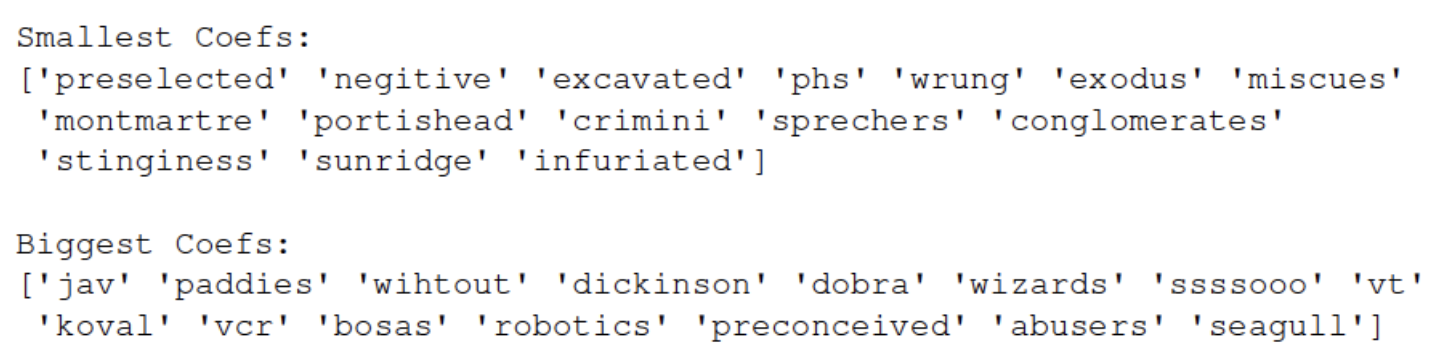
\includegraphics[width=\textwidth]{cowords.png}
\caption{Word features with count vectorizer}
\end{figure}

We sort and show the word features by their coefficients. From Figure 13, we can see that our model built using count vectorizer is not that ideal.We can't observe obvious distinction from the two groups.

\begin{figure}[!h]
\centering
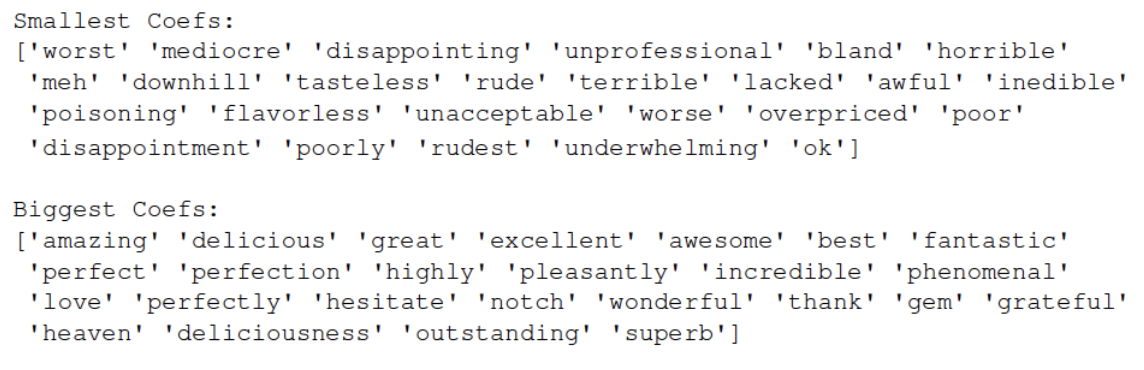
\includegraphics[width=\textwidth]{countwords.png}
\caption{Word features with tf-idf vectorizer}
\end{figure}
The Tf-idf vectorizer performed much better (Figure 14). We can clearly observe that small coefficients are negative words,and larger coefficients are positive words. 

\begin{figure}[!h]
\centering
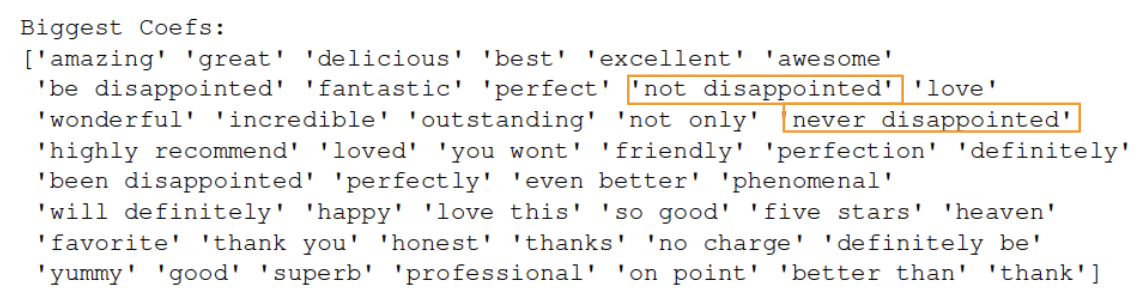
\includegraphics[width=\textwidth]{bigramwords.png}
\caption{Word features with tf-idf vectorizer and bigrams model}
\end{figure}
\begin{figure}[!ht]
\centering
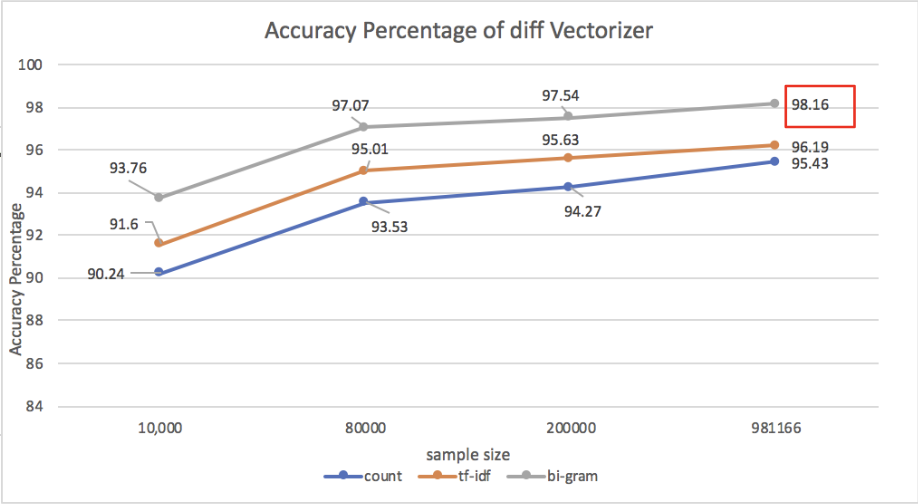
\includegraphics[width=\textwidth]{bigram.png}
\caption{Accuracy percentage of different vectorizer}
\end{figure}
Bigrams (Figure 15) is able to capture negations like "not good" and "not recommend", also compliment like “never disappointed” and "not disappointed". The results showed that including bigrams indeed increased test accuracy (Figure 16).The highest accuracy percentage now is 98.16\% using Tf-idf vectorizer with bigrams model and LinearSVC classification algorithm. 

\section{Future Directions}
\subsection{Multi-classification}
In this section, instead of making a prediction of binary outcome, we try to use "Multi-Naive Bayes", "Bernoulli Naive Bayes", "Logistic Regression", "Stochastic Gradient Descent Classifier", "Support Vector Classifier", "Linear-Support vector Classifier", and "Random Forest Classifier" to predict the review rating from one star to five stars. The overall runtime for predicting five stars review takes much longer to predict the binary outcomes. At first, we start with testing a set of three thousand data points. 1500 data points were set the training set and 1500 data points were set as the testing set. Since we try to make a much accurate prediction, the overall accuracies of seven algorithms are very low, as we can observe from the figure 16. The highest accuracy is 44.40 percentage, which is produced by Logistic Regression. In order to achieve higher accuracy, a set of ten thousand data points were ran. Then five thousand data points were set up as the training set and five thousand data points were set up as the testing set. In general, the accuracy of the algorithm have been increased, except the "Support Vector Classifier." But the accuracies are still very low. At this moment, the runtime becomes much longer. At the end, fifty thousands data points are separated into a twenty-five thousand training set and a twenty-five thousand testing set. The overall accuracies do not increase much. The highest accuracy is 60.70 percentage. 
\begin{figure}[!ht]
\centering
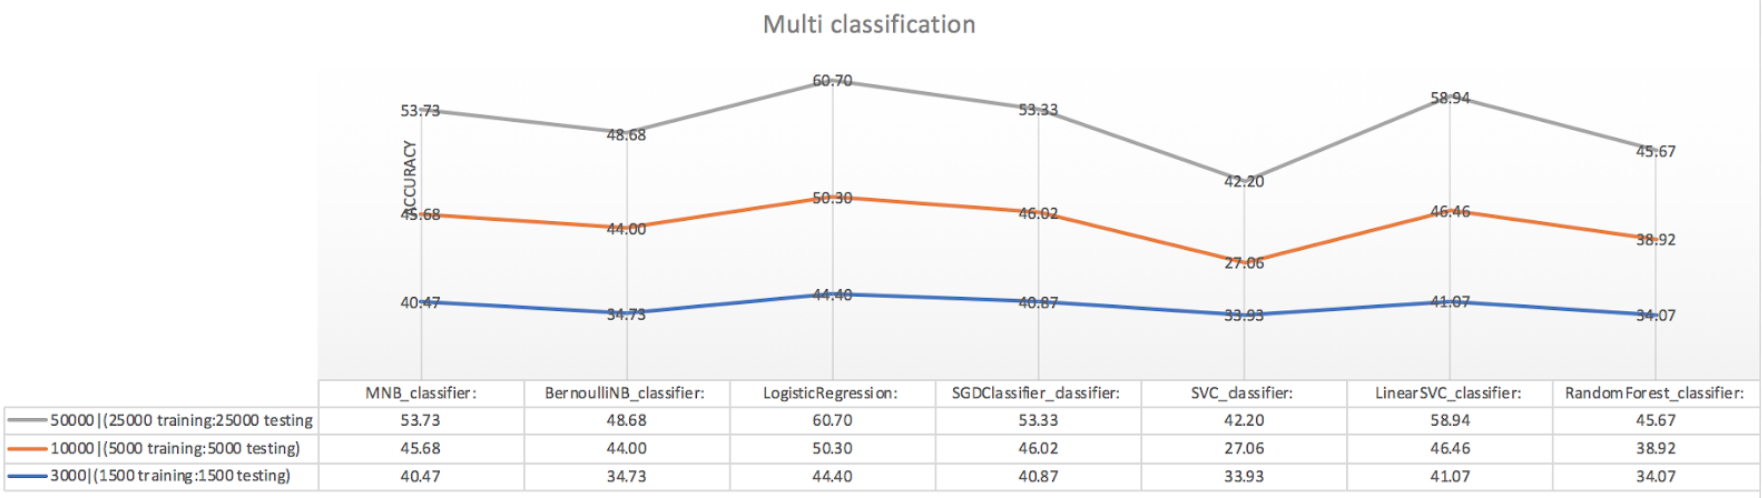
\includegraphics[width=\textwidth]{Multi.png}
\caption{Accuracy percentage of multi-classification}
\end{figure}
\subsection{Building an LDA model}
Topic Modeling is a technique to extract the hidden topics from large volumes of text. Latent Dirichlet Allocation(LDA) is a popular algorithm for topic modeling. LDA’s approach to topic modeling is it considers each document as a collection of topics in a certain proportion. And each topic as a collection of keywords, again, in a certain proportion.Here, we will try to build an LDA model to extract general topics in Yelp's review and explore whether it helps to classify the meaning of the review content. We use Python’s Gensim package to do the implementation and use pyLDAvis package do the visualization of the topics. 

Like the review analysis in section 5, we first prepare the dataset (section 5.1) and preprocess the documents (section 5.2.1). Since two main inputs to the LDA topic model are the dictionary and the corpus, we create the dictionary and corpus using our preprocessed data. 

Before building the LDA model, another big question is that how to find the optimal number of topics $k$. Here, our approach is to find the optimal number of topics is to build many LDA models with different values of number of topics (k) and pick the one that gives the highest coherence value.

\begin{figure}[!ht]
\centering
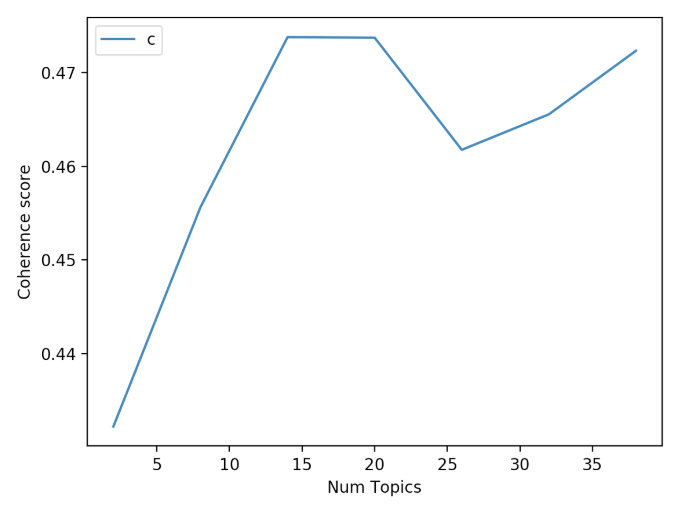
\includegraphics[width=9cm]{k.png}
\caption{Topic coherence score with different number of k}
\end{figure}

Usually, we choose $k$ that marks the end of a rapid growth of topic coherence, which offers meaningful and interpretable topics. From Figure 18, we choose $k$ to be 20. 

We visualize the topics using pyLDAvis package as follows: 
\begin{figure}[!ht]
\centering
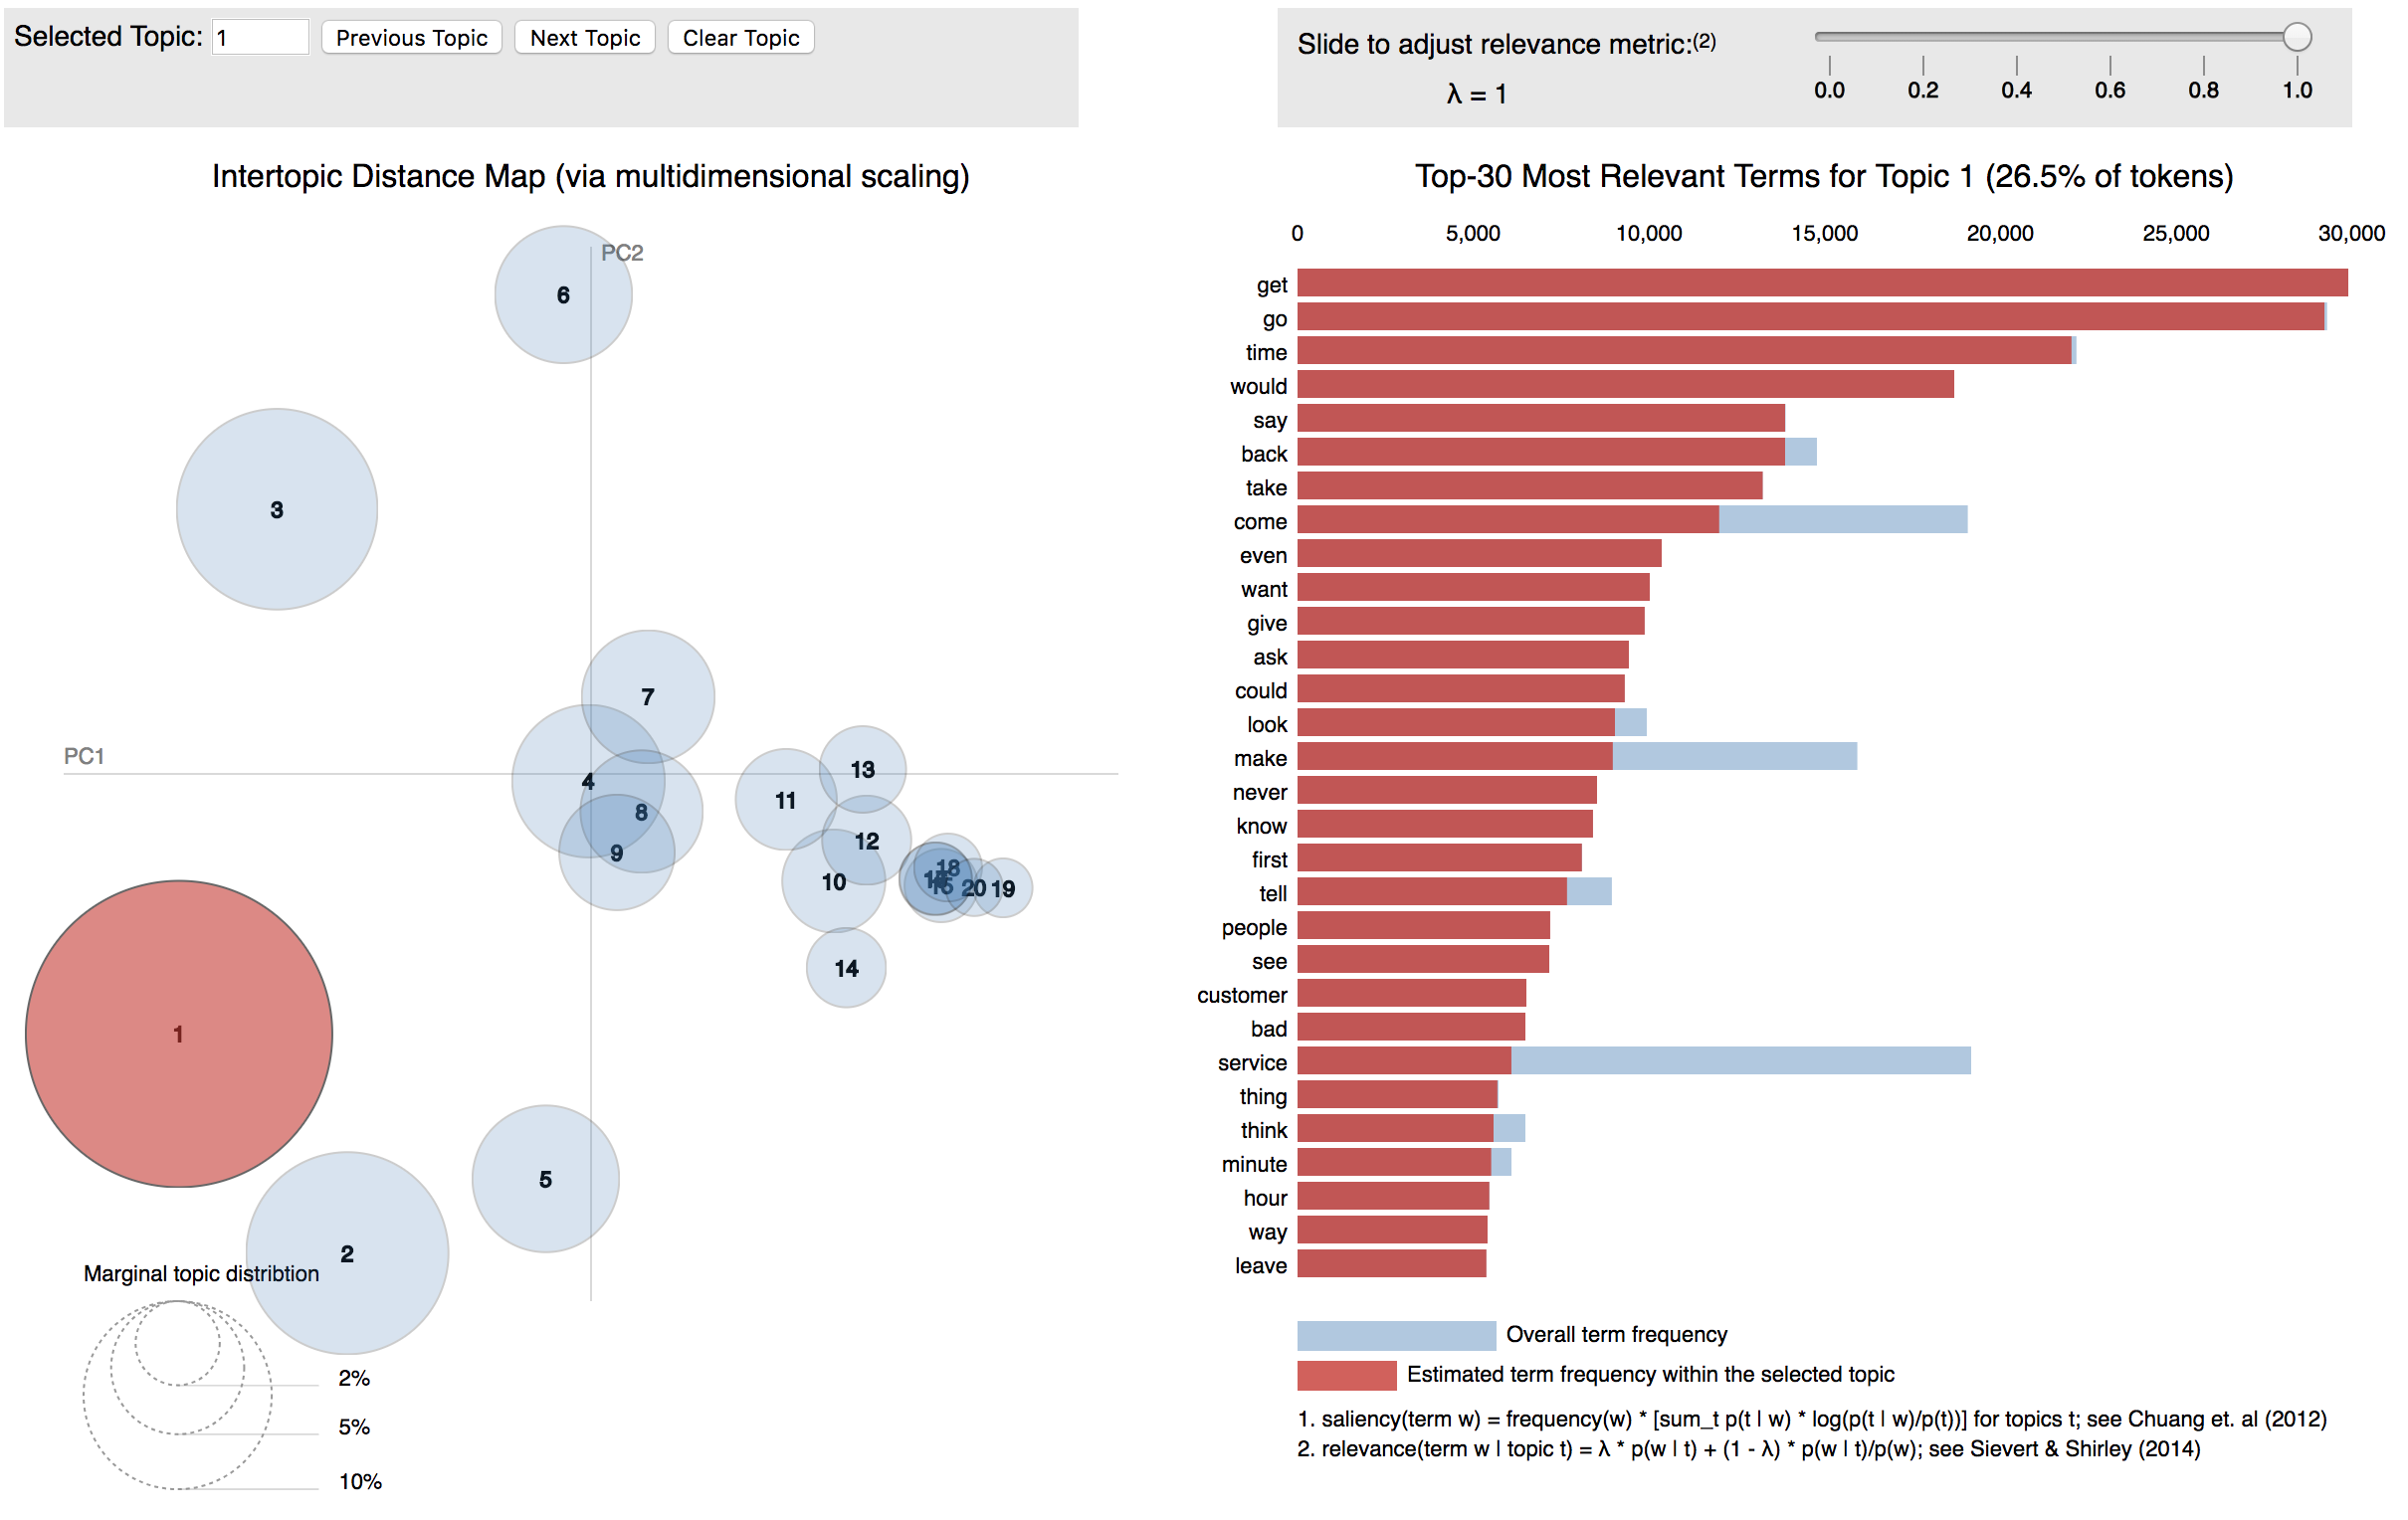
\includegraphics[width=\textwidth]{lda.png}
\caption{topics visualization}
\end{figure}
We can observed that LDA model not performed that well. Using the largest topic 1 as an example, the words showed the topic are mostly verbs which does not convey many meanings and does not help predict the review ratings.

\section{Discussion}
From Figure 16, we observe that larger the dataset, higher the accuracy. The accuracy of predicting the review rating (positive and negative) still can be improved is we use larger data points. 

Recall that in our analysis, we define positive as 4 and 5 stars, negative as 1 and 2 stars. 3 stars are considered neutral and filtered in our analysis. We still need to understand the real insight of dropping the middle rank 3. 

Although the LDA model (section 6.2) we built does not performed well, it can be powerful if carefully designed. The model should be further explored in future analysis.

\section*{References}
[1] https://www.yelp.com/dataset-challenge.

[2] C.J. van Rijsbergen, S.R. and Porter, M. (1980). New models in probabilistic information retrieval. (British Library Research and Development Report, no.5587).

\end{document}


